\providecommand{\main}{..}
\documentclass[\main/notes.tex]{subfiles}

\begin{document}
	\ifSubfilesClassLoaded{\setcounter{chapter}{10}}{}
	\addtocontents{toc}{\protect\newpage}
	\chapter{Data Structure}
		\begin{definition}{Data Structure}
			A collection of related variables that can be accessed individually or as a whole. A set of data items that share s apecific relationship.
		\end{definition}
		\section{Arrays}
			\begin{definition}{Array}
				A sequenced collection of elements of the same data type. Can refer to the elements of the array as the first element, second element, and so on.

				Elements of an array are addressed through their subscripts. \texttt{array[n]} would access the $n$th element of \texttt{array}.
			\end{definition}
			A \concept{multidimensional array} stores arrays inside arrays, in order to store information in rows and columns.
			\subsection{Memory Layout}
				Most computers use \concept{row-major storage}, where an entire row of an array is stored in memory before the next row. However, it may be stored in \concept{column-major storage}, where the entire column is stored before the next column.
			\subsection{Operations on Arrays}
				\begin{definition}{Searching}
					Find the index of an element when the value is known.
				\end{definition}
				\pagebreak
				\begin{definition}{Insertion}
					Add an element to the array.
					\begin{description}
						\item[Insertion at the end] Increase the size of the array, and set \texttt{array[size]} to be the element.
						\item[Insertion at the beginning] If the array needs to be sorted, this can be lengthy and time consuming. Need to search the array to find the index where the element needs to be inserted. Shift every element after that index one towards the end of the array, and then insert the element at the index.
					\end{description}
				\end{definition}
				\begin{definition}{Deletion}
					Remove an element from the array. As lengthy and time consuming as insertion.
				\end{definition}
				\begin{definition}{Retrieval}
					Accessing a particular element from the array. Easy operation, as an array is a \concept{random-access structure}, so each element can be accessed randomly without needing to access the elements before or after.
				\end{definition}
				\begin{definition}{Traversing}
					Apply an operation to all elements of the array, in sequence. Easy operation.
				\end{definition}
			\subsection{Strings}
				\begin{definition}{String}
					A set of characters. Treated differently based on the language. In C, a string is an array of characters. In C++, a string can be an array of characters, or a type. In Java, a String is a type.
				\end{definition}
			\subsection{Application}
				Suitable when the number of deletions and insertions is small, but a lot of searching and retrieval activities are expected.

		\section{Records}
			\begin{definition}{Record}
				A collection of related elements, possibly of different types, that has a single name.

				Each element in a record is called a \concept{field}.
				\begin{indentparagraph}
					\begin{description}
						\item[Field] Smallest element of named data within a record that has meaning. A type that exists in memory -- can be assigned values.
					\end{description}

					Fields are normally referred to after the record, using a period. An example: \texttt{record.field}
				\end{indentparagraph}
				A record defines the identifiable attributes of an element -- it does not define a combination of different elements.
			\end{definition}

		\section{Linked Lists}
			\begin{definition}{Linked List}
				A collection of data in which each element contains the location of the next element. That is, each element contains two parts: the \concept{data} and the \concept{link}. The data holds the information. The link is used to connect the data.

				The \concept{link} contains a \concept{pointer} (an address) that identifies the next element in the list. A pointer is also used to identify the first element in the list. The name of the list is the same as the name of this first pointer.

				The link in the last element contains a \concept{null pointer}, which indicates the end of the list. An empty list is defined to be only a null pointer.

				\begin{center}
					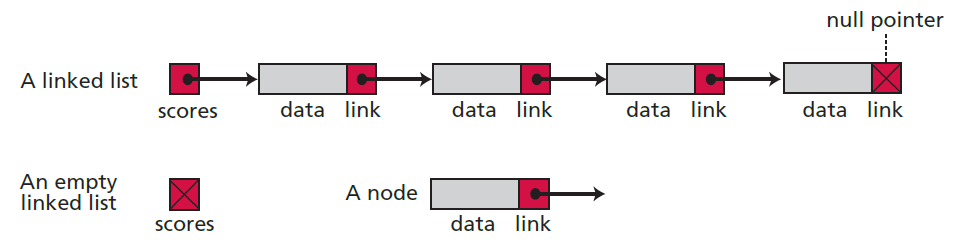
\includegraphics[width=0.9\textwidth]{\main/images/unit11/linked_list.png}
				\end{center}

				The elements in a linked list are called \concept{nodes}. A \concept{node} is a record that has at least two fields: one containing the data, and the other containing the address of the next node in the sequence.
			\end{definition}
			Both arrays and linked lists are representations of a list of items in memory. The different is the way the items are linked together. In an array, this is through the \concept{index}. In a linked list, this is through the link that points to the next element.
			\begin{center}
				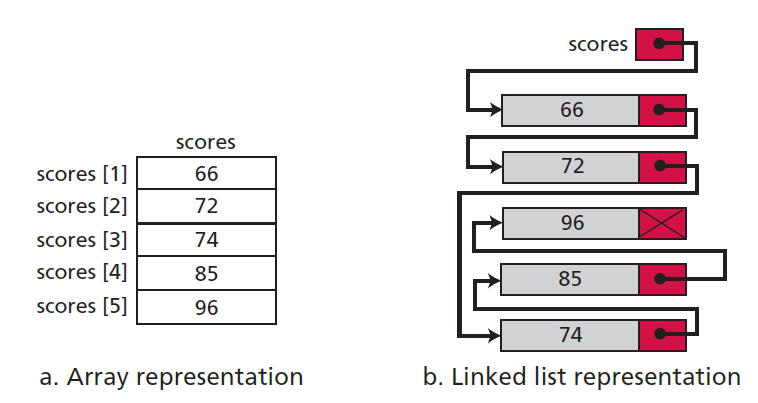
\includegraphics[width=0.6\textwidth]{\main/images/unit11/array_v_linked_list.png}
			\end{center}
			The elements of an array are stored right after each other in memory -- the list is contiguous. The nodes of a linked list can be stored with gaps between them. This means insertion and deletion is easier. But this means each node needs to have an extra field to store the address.

			The name of a linked list is the name of the head pointer that points to the first node on the list. Nodes do not have explicit names, just implicit ones. The name of a node is related to the name of the pointer that points to the node. The convention used in the C language is that, if a pointer that points to a node is called \texttt{p}, then the node is called \texttt{*p}. As the node is a record, the fields inside it can be accessed using the name of the node. \texttt{(*p).data} and \texttt{(*p).link}
			\subsection{Operations on Linked Lists}
				\begin{definition}{Searching}
					Can only be sequential, as the nodes in a linked list have no specific names that can be dound using a binary search.

					As nodes have no names, two pointers are used: \texttt{pre} (for previous), and \texttt{cur} (for current). The search algorithm moves the two pointers together towards the end of the list.
					\begin{center}
						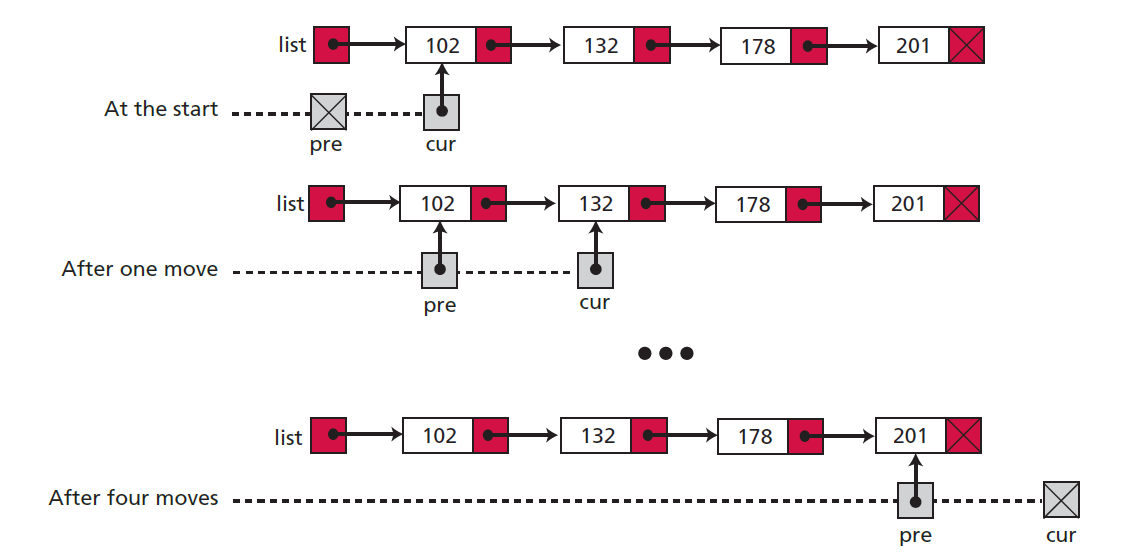
\includegraphics[width=0.7\textwidth]{\main/images/unit11/linked_list_moving_pointers.png}
					\end{center}

					When the search stops, the \texttt{cur} pointer points to the node that stops the search, and the \texttt{pre} pointer points to the previous node. If the target is found, \texttt{cur} points to the node that holds the target value. If the target value is not found, \texttt{cur} points to the node with a larger value than the target value.

					The searching algorithm uses a \concept{flag} that marks whether the target is found or not. If the flag is true, then the target was found, and \texttt{cur} points to the target. If the flag is false, then the target was not found, and \texttt{cur} points to a value larger than the target.

					\begin{center}
						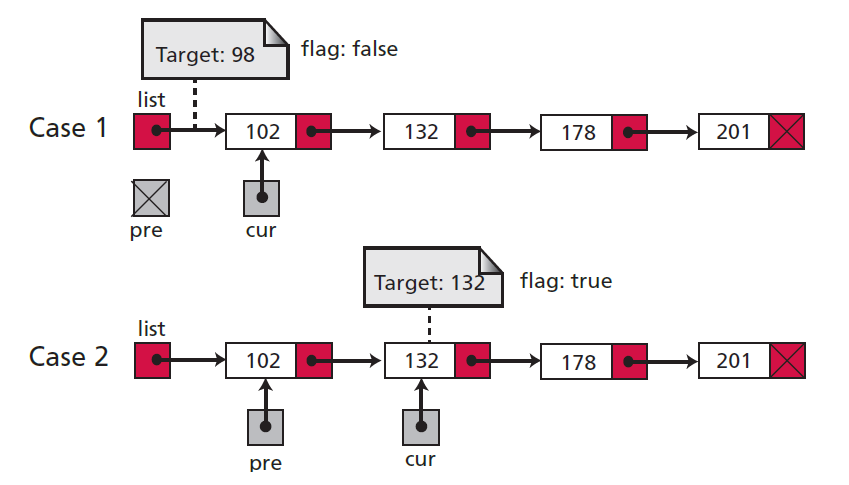
\includegraphics[width=0.7\textwidth]{\main/images/unit11/linked_list_search_cases_1.png}
						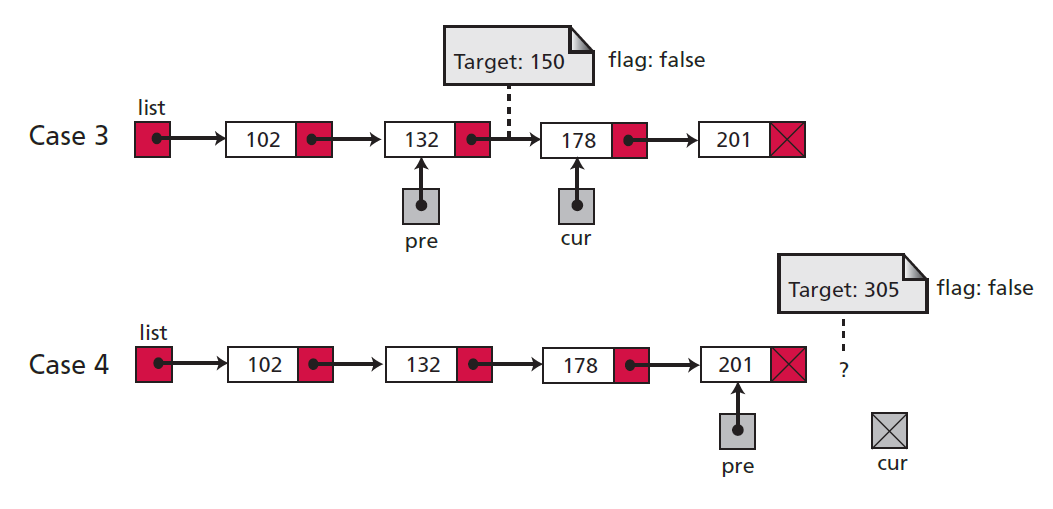
\includegraphics[width=0.9\textwidth]{\main/images/unit11/linked_list_search_cases_2.png}
					\end{center}
				\end{definition}
				\begin{definition}{Inserting a Node}
					First apply the searching algorithm, in case the value is already present, as duplicate values are not allowed. In that case, there are four possibilities:
					\begin{indentparagraph}
						\begin{description}
							\item[Inserting into an empty list] Insert the new item as the first element.
								\begin{lstlisting}
list <- new
								\end{lstlisting}
							\item[Inserting at the beginning] If the search algorithm has a flag of \texttt{false}, and the value of \texttt{pre} is null, then the data needs to be inserted at the start.
								\begin{lstlisting}
(*new).link <- cur
list <- new
								\end{lstlisting}
							\item[Inserting at the end] If the search algorithm has a flag of \texttt{false}, and the value of \texttt{cur} is null, then the data needs to be inserted at the end.
								\begin{lstlisting}
(*pre).link <- new
(*new).link <- null
								\end{lstlisting}
							\item[Inserting in the middle] If the search algorithm has a flag of \texttt{false}, and neither \texttt{pre} nor \texttt{cur} is null, then the data needs to be inserted in the middle.
								\begin{lstlisting}
(*new).link <- cur
(*pre).link <- new
								\end{lstlisting}
						\end{description}
					\end{indentparagraph}
				\end{definition}
				\pagebreak
				\begin{definition}{Deleting a Node}
					First apply the searching algorithm. If the flag is false, the node is not present. Otherwise, the node can be deleted. Easier than insertion: only two cases -- deleting the first node, and deleting any other node.
					\begin{indentparagraph}
						\begin{description}
							\item[Deleting the first node] If the \texttt{pre} pointer is null, the first node needs to be deleted. The \texttt{cur} pointer points to the first node, and deleting can be done in one statement:
								\begin{lstlisting}
list <- (*cur).link
								\end{lstlisting}
							\item[Deleting any other node] If neither of the pointers is null, the node to be deleted is either a middle node or the last node. The \texttt{cur} pointer points to the node to be deleted. Deleting can be done in one statement:
								\begin{lstlisting}
(*pre.link) <- (*cur).link
								\end{lstlisting}
						\end{description}
					\end{indentparagraph}
				\end{definition}
				\begin{definition}{Retrieving a Node}
					Randomly accessing a node for the purpose of inspecting or copying the data contained in the node. The linked list needs to be searched. If the item is found, it is retreived, otherwise it is aborted.

					Much simpler than insertion or deletion -- uses only the \texttt{cur} pointer, which will point to the node found by the search algorithm.
				\end{definition}
				\begin{definition}{Traversing a Linked List}
					Use a `walking' pointer -- a pointer that moves from node to node as each element is processed. Start by setting the walking pointer to the first node in the list, and then use the links of the different nodes until all the data has been processed. When the last node is processed, the walking pointer will become null, and the process will terminate.
				\end{definition}
			\subsection{Application of Linked Lists}
				Efficient for storing data that will go through many insertions and deletions. A dynamic data structure that can easily grow and shrink. The overhead is needing to hold an extra field for each node.

				Not efficient for data that must be searched often -- an array is faster for searching.

	\rulechapterend

\end{document}